\documentclass[11pt]{article}


\RequirePackage{vruler}
\usepackage{crop}%
\usepackage{amsmath,amssymb,amsfonts,upref,endnotes}
\usepackage{amsthm}
\usepackage{marginnote}
\usepackage{soul}
\RequirePackage{graphicx}
\usepackage[figuresright]{rotating}
\usepackage{color}
\usepackage{lineno}
\usepackage{siunitx}
\usepackage[colorinlistoftodos,textsize=small,textwidth=3.75cm,color=yellow]{todonotes}


\renewcommand{\figurename}{Figure. S}

\linenumbers

\usepackage{dcolumn}
\newcolumntype{d}{D{.}{.}{-1}}

\RequirePackage[T1]{fontenc}

\usepackage{palatino}
\usepackage[scaled=0.85]{helvet}



\begin{document}


\linespread{1}\selectfont %Single spacing


\begin{figure}[!h]
\centering
	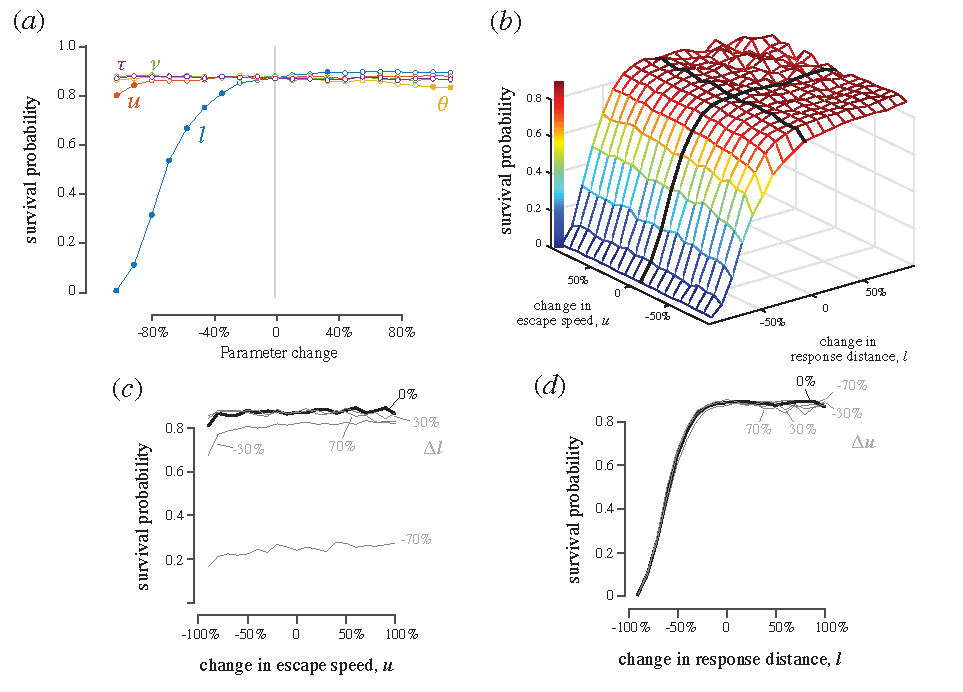
\includegraphics[width=5.5in]{supp_sense}
\caption{Sensitivity analysis of the probabilistic, agent-based model with a juvenile predator. 
(\textit{a}) We varied the mean of the distribution for each prey parameter by manipulating the log-mean value (see Table 1 for parameter definitions and values), with each point representing the result of 1000 simulations. 
Solid points represent significant differences (KS-test: P < 0.05) from a 0\% change.
(\textit{b}) Variation in escape probability was examined with respect to both escape speed and reaction distance.
The same simulation results are shown with respect to changes in escape speed (\textit{c}) and reaction distance (\textit{d}).
}
\label{fig_sense}
\end{figure}

\begin{figure}[!h]
\centering
	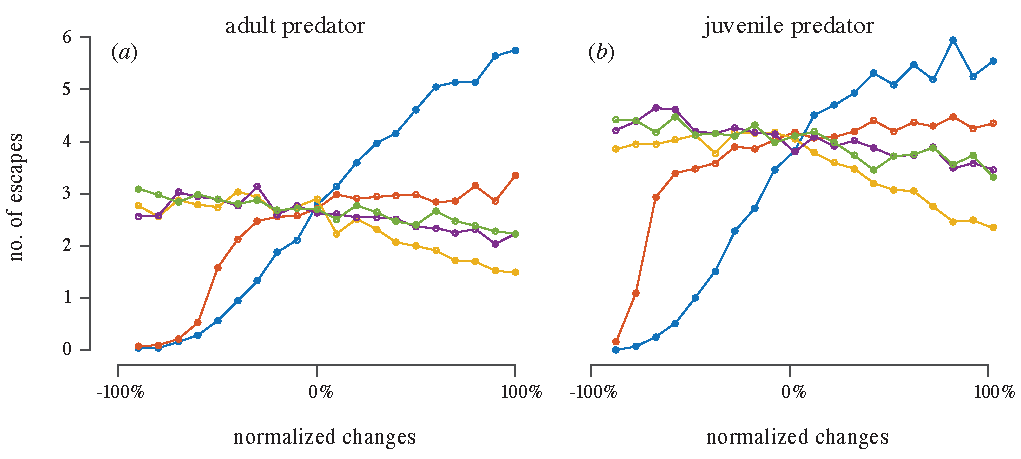
\includegraphics[width=5.5in]{supp_noescape}
\caption{The number of escapes prior to capture generated by the sensitivity analysis of the probabilistic, agent-based model.
These are the sample simulations from which survival probability was determined with respect to differences in parameter values for (\textit{a}) juvenile predators (same simulations as in Fig. S1\textit{a}) and (\textit{b}) adult (same simulations as in Fig. 4\textit{a}).
The shapes of these curves are different from when they are presented as survival probability because a probability cannot exceed a value of unity.
}
\label{fig_sense}
\end{figure}

\begin{figure}[!h]
\centering
	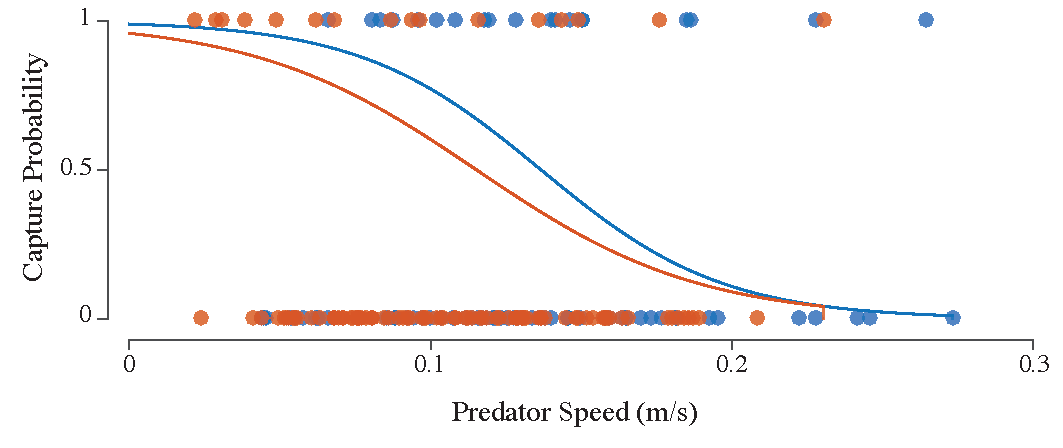
\includegraphics[width=5.5in]{supp_pred_speed_vs_capture}
\caption{Logistical regression between predator speed and the probability of prey capture.
Each point on this plot represent an approach by the predator with its corresponding speed.
A value of 1 represents a successful capture by the predator; while a value of 0 represents a failed capture. 
A logistical regression was taken the for points present, with the data in orange representing the juvenile zebrafish observations and the data in blue representing adult zebrafish observations.
For either predator, there was greater chance of capturing prey, when predators approached with a lower speed.
}
\label{fig_sense}
\end{figure}

\begin{figure}[!h]
\centering
	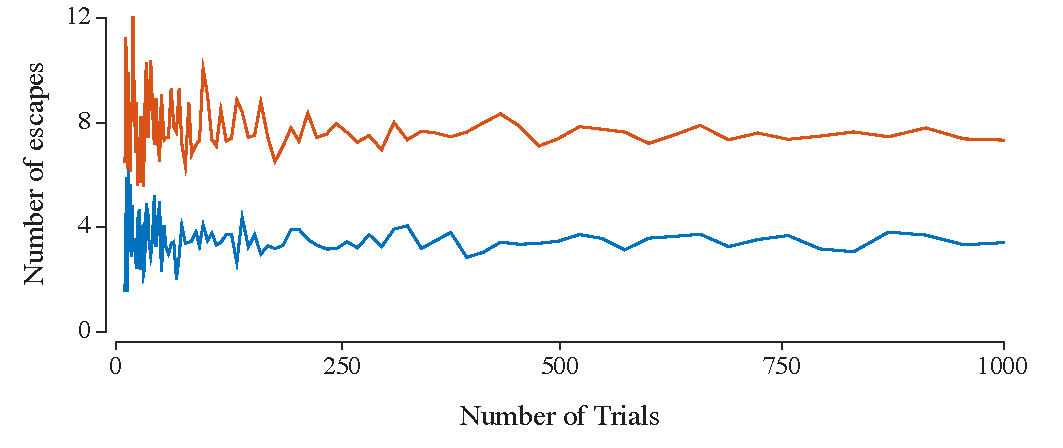
\includegraphics[width=5.5in]{supp_num_trials}
\caption{The average number of escapes over a varying amount of trails.
As a monte-carlo simulation, the probabilistic, agent-based model was ran a varying amount of times to see how the results would vary.
1000 trails is well beyond where the trend stabilizes.
}
\label{fig_sense}
\end{figure}

\end{document}


